\section{¿Afecta en la nota el consumo de alcohol?}

En nuestra muestra hay 244 alumnos que consumen alcohol los fines de semana (un 62\%), de los cuales la media de edad es de $16.8$ años (es decir, la mayoría son menores). Es probable que en estas edades los alumnos aun no gestionen bien el consumo de alcohol y es posible que esto repercuta en sus notas finales.
\begin{equation*}
    \begin{split}
        & X \equiv \text{Nota final de los alumnos que consumen alcohol los fines de semana}\\
        & Y \equiv \text{Nota final de los alumnos que no consumen alcohol los fines de semana}
    \end{split}
\end{equation*}

En nuestros datos si que observamos un descenso en la nota media de los alumnos que consumen alcohol.
\begin{equation*}
    \begin{split}
        & \bar{x} = 10.22\\
        & \bar{y} = 10.74
    \end{split}
\end{equation*}

\begin{figure}[H]
    \begin{center}
        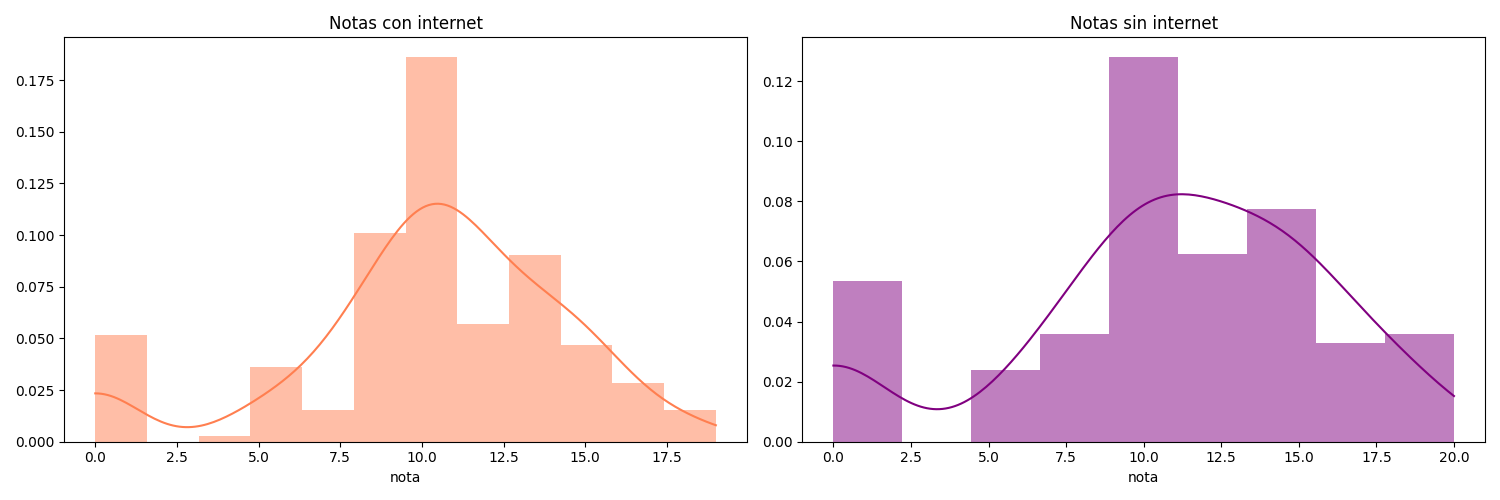
\includegraphics[width=1\textwidth]{figures/dist-notas-walc.png}
    \end{center}
    \caption{Gráficos de distribución de la nota final de los alumnos que consumen alcohol los fines de semana y de los que no}\label{fig:dist-notas-walc}
\end{figure}

Si estudiamos el QQ-plot de las notas finales de ambos grupos, obtendremos resultados similares al anterior: existen muchos \textit{outliers} de los alumnos que no se presentaron al examen final.
\begin{figure}[H]
    \begin{center}
        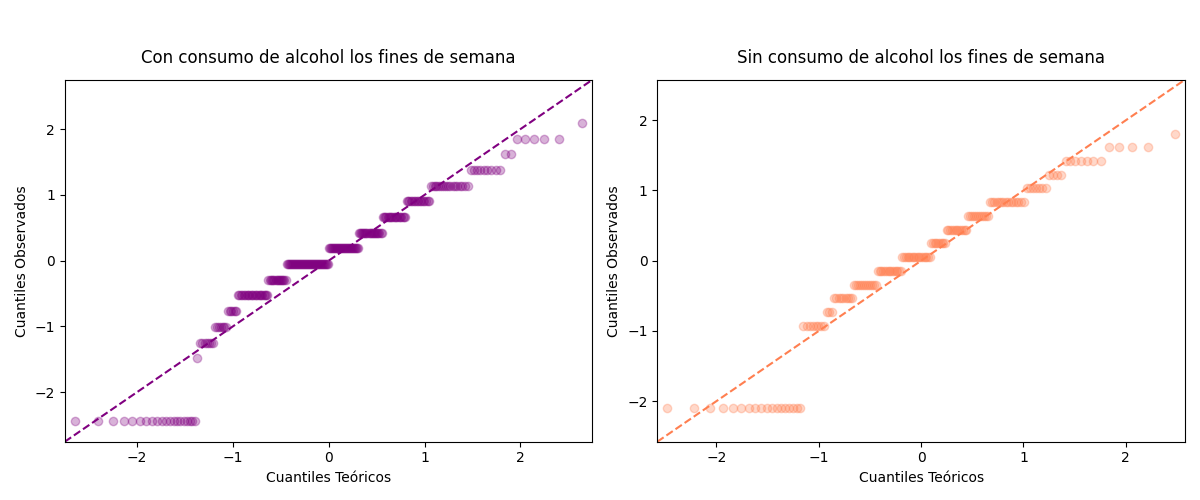
\includegraphics[width=1\textwidth]{figures/qq-plot-walc.png}
    \end{center}
    \caption{QQ-plot de la nota final de los alumnos que consumen alcohol los fines de semana y de los que no}\label{fig:qq-plot-walc}
\end{figure}

Si comprobamos la asimetría de la muestras veremos que es moderada en ambos casos.
\begin{equation*}
    \begin{split}
        & \gamma_{1}(x) = \frac{\sum_{i=1}^{n}(x_i - \bar{x})^3}{n \cdot s^3} = -0.82\\
        & \gamma_{1}(y) = \frac{\sum_{i=1}^{n}(y_i - \bar{y})^3}{n \cdot s^3} = -0.70
    \end{split} 
\end{equation*}

Por lo tanto, como además estamos trabajando con muestras grandes e independientes, utilizaremos un contraste paramétrico de diferencia de medias para muestras grandes independientes con varianzas poblacionales desconocidas (Z test).
\begin{itemize}
    \item \textbf{Hipótesis nula ($H_0$)}: $\mu_x - \mu_y = 0$ (no existen diferencias significativas entre la media de las notas finales de los alumnos que consumen alcohol los fines de semana y de los que no)
    \item \textbf{Hipótesis alternativa ($H_a$)}: $\mu_x - \mu_y < 0$ (la nota media de los alumnos que consumen alcohol los fines de semana es significativamente menor que la de los alumnos que no consumen)
\end{itemize}

Al calcular el estadístico de contraste $Z_{\text{obs}}$, obtenemos el siguiente p-valor.
\begin{equation}
    Z_{\text{obs}} = -1.09 \Rightarrow \text{p-valor} = P(Z < -1.09) = 0.14
\end{equation}

Si fijamos un nivel de significación $\alpha = 0.05$ (el error de tipo 1 máximo que permitimos en nuestro contraste), entonces $\text{p-valor} > \alpha$ lo que significa que al 5\% los datos no dan evidencias suficientes como para rechazar que las medias de las notas finales de los alumnos que consumen y no consumen alcohol los fines de semana sean iguales. Por lo tanto, al 5\% aceptaremos que las notas medias de los alumnos que toman y no toman alcohol no difieren significativamente.
